\chapter{Ondas electromagnéticas}
Las ecuaciones de Maxwell muestran que un campo magnético variable en el tiempo actúa como fuente de campo eléctrico, y que un campo eléctrico que varía con el tiempo genera un campo magnético. Estos campos $\vec{E}$ y $\vec{B}$ se sostienen uno al otro y forman una onda electromagnética que se propaga a través del espacio.

A diferencia de las ondas en una cuerda o las del sonido en un fluido, las ondas electromagnéticas no requieren un medio material.

\section{Ecuaciones de Maxwell y ondas electromagnéticas}
La ley de Faraday plantea que un campo magnético variable en el tiempo actúa como fuente de campo eléctrico, como lo demuestran las fem inducidas en los inductores y transformadores.

La ley de Ampère,  afirma que un campo eléctrico que cambia con el tiempo actúa como una fuente de campo magnético. Esta interacción mutua entre los dos campos se resume en las ecuaciones de Maxwell.

Así, cuando un campo, \textit{ya sea} eléctrico o magnético, cambia con el tiempo, induce un campo del otro tipo en las regiones adyacentes del espacio.

\subsection{Electricidad, magnetismo y luz}
Maxwell descubrió que los principios básicos del electromagnetismo podían expresarse en términos de las cuatro ecuaciones que hoy conocemos como \textbf{ecuaciones de Maxwell}. Estas cuatro ecuaciones son: 1) la ley de Gauss de los campos eléctricos; 2) la ley de Gauss de los campos magnéticos, que demuestra la inexistencia de monopolos magnéticos; 3) la ley de Ampère, que incluye la corriente de desplazamiento; y 4) la ley de Faraday:

\begin{equation}\label{29.18}\marginnote{Ley de Gauss}
\oint\vec{E}\cdot\, d\vec{A}=\frac{Q_{enc}}{\epsilon_0}
\end{equation}
\begin{equation}\label{29.19}\marginnote{Ley de Gauss del magnetismo}
\oint\vec{B}\cdot\, d\vec{A}=0
\end{equation}
\begin{equation}\label{29.20}\marginnote{Ley de Ampère}
\oint\vec{B}\cdot\, d\vec{l}=\mu_0\left(i_C+\epsilon_0\frac{d\Phi_E}{dt}\right)_{enc}
\end{equation}
\begin{equation}\label{29.21}\marginnote{Ley de Faraday}
\oint\vec{E}\cdot\, d\vec{l}=-\frac{d\Phi_B}{dt}
\end{equation}

Estas ecuaciones se aplican a los campos eléctricos y magnéticos \textit{en el vacío}. Si está presente un material, la permitividad $\epsilon_0$ y la permeabilidad $\mu_0$ del espacio libre se sustituyen por la permitividad $\epsilon$ y la permeabilidad $\mu$ del material. Si los valores de $\epsilon$ y $\mu$ son diferentes en puntos distintos en las regiones de integración, entonces $\epsilon$ y $\mu$ deben transferirse al lado izquierdo de (\ref{29.18}) y (\ref{29.20}), respectivamente, y colocarse dentro de las integrales. El término $\epsilon$ en (\ref{29.20}) también tiene que incluirse en la integral cuyo resultado es $d\Phi_B/dt$.

De acuerdo con las ecuaciones de Maxwell, una carga puntual en reposo produce
un campo $\vec{E}$ estático pero no un campo $\vec{B}$; una carga puntual en movimiento con velocidad constante produce los dos campos $\vec{E}$ y $\vec{B}$. Las ecuaciones de Maxwell también se usan para demostrar que para que una carga puntual produzca ondas electromagnéticas, la carga debe \textit{acelerar}. De hecho, un resultado general de las ecuaciones de Maxwell es que toda carga acelerada irradia energía electromagnética.

\subsection{Generación de la radiación electromagnética}
Una manera de conseguir que una carga puntual emita ondas electromagnéticas es haciéndola oscilar en movimiento armónico simple, de manera que tenga una aceleración casi en todo instante (excepto cuando la carga pasa por la posición de equilibrio).

Puesto que las perturbaciones eléctricas y magnéticas se dispersan o irradian desde la fuente, se utiliza de manera indistinta el nombre de \textbf{radiación electromagnética} o el de “ondas electromagnéticas”.

El físico alemán Heinrich Hertz, una vez que determinó la frecuencia de resonancia de sus circuitos, encontró la rapidez de las ondas a partir de la relación entre su longitud de onda y su frecuencia, $v=\lambda f$, y estableció que era igual a la rapidez de la luz. El valor moderno de la rapidez de la luz, que se denota con el símbolo $c$, es $299,792,458$ [m/s]. Para nuestros propósitos, el valor de $3.00 \times 10^8$ [m/s] tiene suficiente exactitud.

\subsection{El espectro electromagnético}
 El \textbf{espectro electromagnético} de las ondas electromagnéticas incluye las ondas de radio y televisión, la luz visible, la radiación infrarroja y ultravioleta, los rayos x y los rayos gamma.
 
A pesar de las muchas diferencias en su uso y medios de producción, todas ellas las ondas electromagnéticas tienen la misma rapidez de propagación (en el vacío), $c=299,792,458$ [m/s]. Las ondas electromagnéticas difieren en frecuencia $f$ y longitud de onda $\lambda$, pero la relación $c=\lambda f$ en el vacío se cumple para cada una.

Nosotros sólo podemos detectar directamente una parte muy pequeña del espectro con nuestro sentido de la vista, y a ese intervalo lo denominamos \textbf{luz visible}\footnote{La radiación electromagnética con la longitud de onda más corta, los rayos gamma, es producida en la naturaleza por los materiales radiactivos.}. Su intervalo de longitud de onda va de $400$ a $700$ nm ($400$ a $700\times 10^{-9}$ [m]), con frecuencias correspondientes de $750$ a $430$ THz ($7.5$ a $4.3\times 10^{14}$ [Hz]) aproximadamente.  Las distintas partes del espectro visible evocan en los humanos las sensaciones de los diferentes colores.

%\begin{figure}
%\centering
%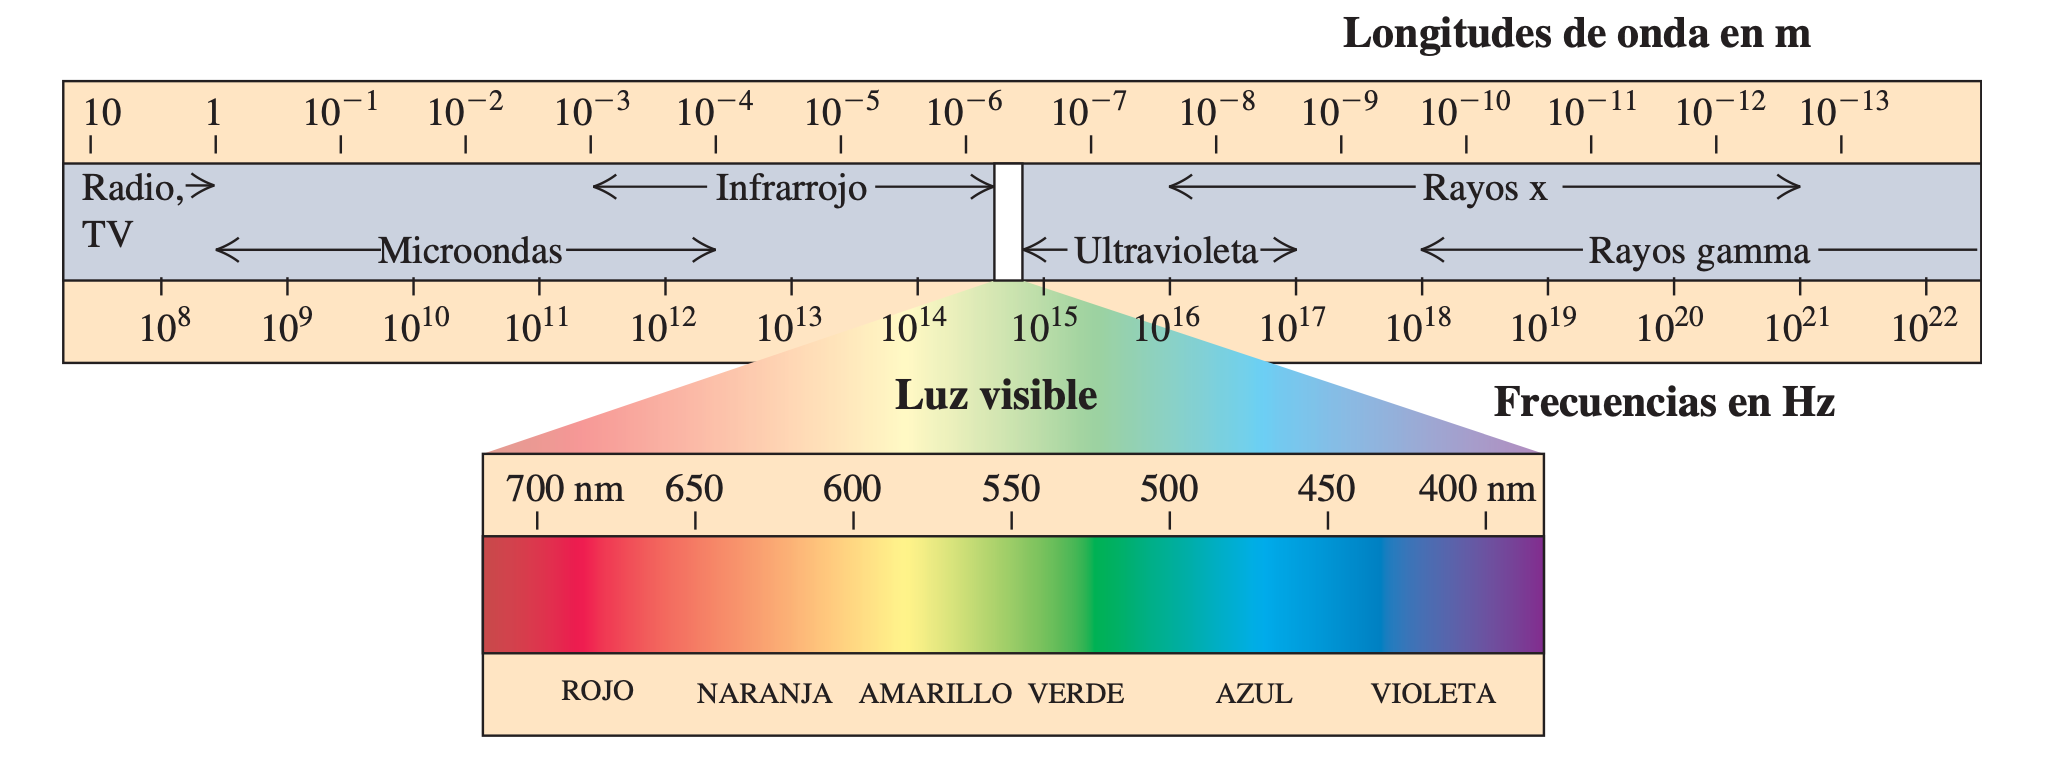
\includegraphics[scale=0.5]{fig/espectro}
%\caption{El espectro electromagnético. Las frecuencias y longitudes de onda que se encuentran en la naturaleza se extienden en un intervalo tan amplio que se tiene que usar una escala logarítmica para i%ndicar todas las bandas importantes. Las fronteras entre las bandas son un tanto arbitrarias.}
%\label{fig:espectro}
%\end{figure}

\section{Ondas electromagnéticas planas y rapidez de la luz}
Nuestro procedimiento consistirá en postular una configuración simple de campo eléctrico que tenga un comportamiento ondulatorio. Supondremos un campo eléctrico $\vec{E}$ que tenga sólo una componente $y$, y un campo magnético $\vec{B}$ sólo con una componente $z$, y supondremos que ambos campos se mueven juntos en la dirección $+x$ con una rapidez $c$ que al principio es desconocida

\subsection{Una onda electromagnética plana simple}

\begin{figure}[h]
\centering
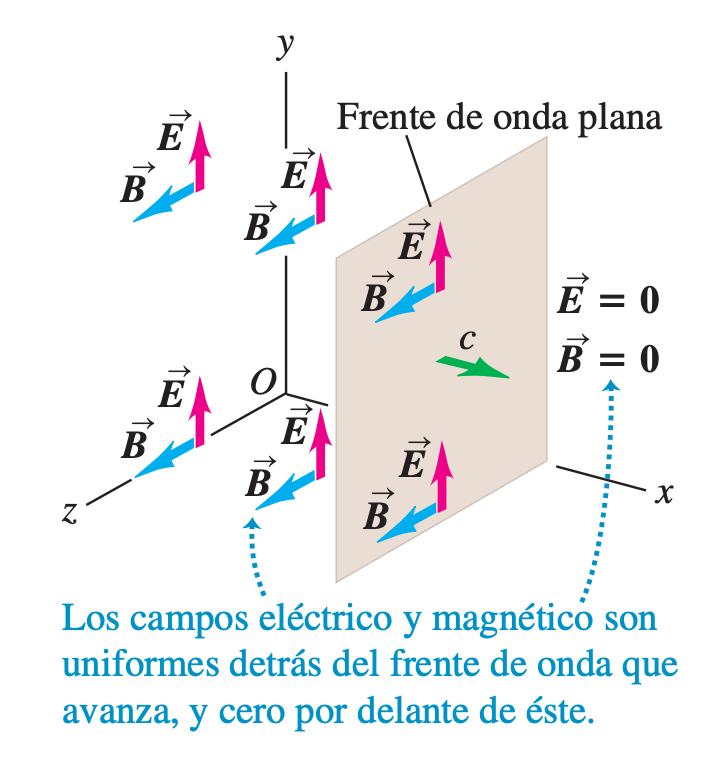
\includegraphics[scale=0.4]{fig/oeps}
\caption{Frente de una onda electromagnética.}
\label{fig:oeps}
\end{figure}

Si tomamos como base un sistema de coordenadas $xyz$ (figura \ref{fig:oeps}), suponemos que todo el espacio está dividido en dos regiones por un plano perpendicular al eje $x$ (y paralelo al plano $yz$). En cada punto a la izquierda de este plano hay un campo eléctrico uniforme $\vec{E}$ en la dirección $+y$ y un campo magnético uniforme $\vec{B}$ en la dirección $+z$, como se ilustra. Además supongamos que el plano limítrofe, al que llamaremos \textit{frente de onda}, se desplaza hacia la derecha en la dirección $+x$ con rapidez constante $c$, un valor que por el momento dejaremos indeterminado. Así, los campos $\vec{E}$ y $\vec{B}$ viajan a la derecha hacia regiones hasta ahora libres de campo con rapidez definida. En resumen, la situación describe una onda electromagnética rudimentaria. Una onda como ésta, en la que en cualquier instante los campos son uniformes en toda la extensión de cualquier plano perpendicular a la dirección de propagación, se llama \textbf{onda plana}. En el caso que se ilustra en la figura \ref{fig:oeps}, los campos son igual a cero para los planos que están a la derecha del frente de onda y tienen los mismos valores en todos los planos ubicados a la izquierda del frente de onda.

Verifiquemos si nuestra onda satisface la primera y segunda ecuaciones de Maxwell, es decir, las leyes de Gauss de los campos eléctrico y magnético. Para ello, tomaremos como nuestra superficie gaussiana una caja rectangular con lados paralelos a los planos coordenados $xy, xz$ y $yz$. La caja no encierra cargas eléctricas. Se puede demostrar que los flujos eléctrico y magnético totales a través de la caja son iguales a cero. Esto \textit{no} sería el caso si $\vec{E}$ o $\vec{B}$ tuvieran una componente $x$, paralela a la dirección de propagación. Así, para satisfacer las ecuaciones primera y segunda de Maxwell, los campos eléctrico y magnético deben ser perpendiculares a la dirección de propagación; es decir, la onda debe ser \textbf{transversal}.

La siguiente ecuación de Maxwell por considerar es la ley de Faraday:

\begin{equation}\label{32.1}
\oint\vec{E}\cdot\, d\vec{l}=-\frac{d\Phi_B}{dt}
\end{equation}

\begin{figure}[h]
\centering
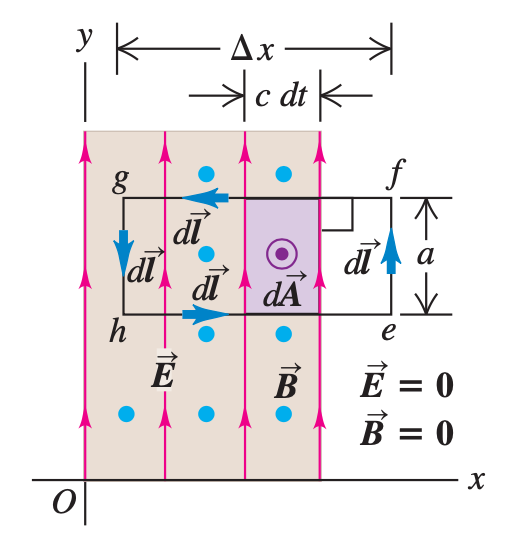
\includegraphics[scale=0.5]{fig/lf}
\caption{En el momento $dt$, el flujo magnético a través del rectángulo en el plano $xy$ se incrementa en una cantidad $d\Phi_B$. Este incremento es igual al flujo a través del rectángulo sombreado, con área $ac\, d$t; es decir, $d\Phi_B=Bac\, dt$. Por lo tanto, $d\Phi_B/dt=Bac$.}
\label{fig:lf}
\end{figure}

Para probar si nuestra onda satisface la ley de Faraday, aplicamos esta ley a un rectángulo $efgh$ paralelo al plano $xy$, el cual tiene altura $a$ y anchura $\Delta x$ (fugura \ref{fig:lf}). En el instante que se ilustra, el frente de onda ha avanzado parcialmente a través del rectángulo, y $\vec{E}$ es igual a cero a lo largo del lado $ef$. Al aplicar la ley de Faraday suponemos que el área vectorial $\vec{A}$ del rectángulo $efgh$ está en la dirección $+z$. Sólo el lado $gh$ contribuye a la integral, y sobre él $\vec{E}$ y $d\vec{l}$ son opuestos, por lo que se obtiene

\begin{equation}\label{32.2}
\oint\vec{E}\cdot\, d\vec{l}=-Ea
\end{equation}

Por consiguiente, el lado izquierdo de (\ref{32.2}) es diferente de cero.

Para satisfacer la ley de Faraday, (\ref{32.1}), debe haber una componente de $\vec{B}$ en la dirección $z$ (perpendicular a $\vec{E}$) de manera que pueda haber un flujo magnético $\Phi_B$ distinto de cero a través del rectángulo $efgh$ y una derivada $d\Phi_B/dt$ diferente de cero. En realidad, nuestra onda $\vec{B}$ tiene sólo la componente $z$. Durante un intervalo de tiempo $dt$, el frente de onda se desplaza una distancia $c\, dt$ hacia la derecha en la figura \ref{fig:lf}, y recorre un área $ac\, dt$ del rectángulo $efgh$. Durante este intervalo, el flujo magnético $\Phi_B$ a través del rectángulo $efgh$ se incrementa en $d\Phi_B =B(ac\, dt)$, por lo que la tasa de cambio del flujo magnético es

\begin{equation}\label{32.3}
\frac{d\Phi_B}{dt}=Bac
\end{equation}

Sustituyendo (\ref{32.2}) y (\ref{32.3}) en (\ref{32.1}), obtenemos

\begin{equation*}
-Ea=Bac
\end{equation*}
\begin{equation}\label{32.4}\marginnote{Onda electromagnética en el vacío}
\boxed{E=cB}
\end{equation}

Así, se ha demostrado que nuestra onda es congruente con la ley de Faraday sólo si su rapidez $c$ y las magnitudes de los vectores $\vec{E}$ y $\vec{B}$ guardan la relación que describe (\ref{32.4}).

Por último, se hace un cálculo similar empleando la ley de Ampère, el miembro restante de las ecuaciones de Maxwell. No hay corriente de conducción $(iC = 0)$, por lo que la ley de Ampère es

\begin{equation}\label{32.5}
\oint\vec{B}\cdot d\,\vec{l}=\mu_0\epsilon_0\frac{d\Phi_E}{dt}
\end{equation}

\begin{figure}[h]
\centering
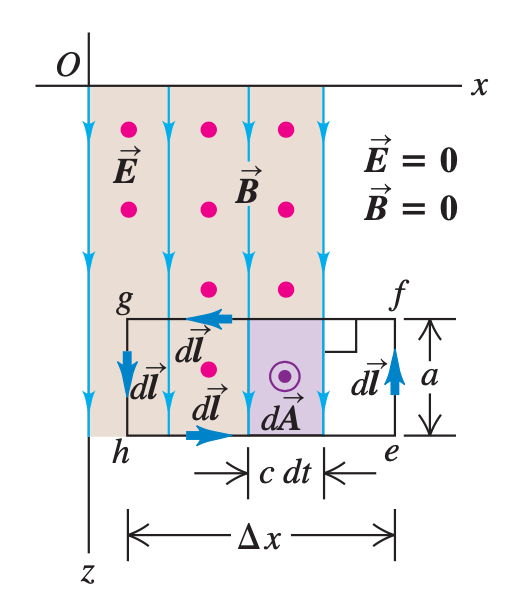
\includegraphics[scale=0.5]{fig/la}
\caption{Aplicación de la ley de Ampère
a una onda plana.}
\label{fig:la}
\end{figure}

Movemos nuestro rectángulo de manera que esté sobre el plano $xz$, como se ilustra en la figura \ref{fig:la}, y de nuevo observamos la situación en un momento en que el frente de onda haya viajado parcialmente a través del rectángulo. Tomamos el área vectorial $d\vec{A}$ en la dirección $+y$. Sólo el lado $gh$, donde $\vec{B}$ y $d\, \vec{l}$ son paralelos, contribuye a la integral, por lo que se obtiene

\begin{equation}\label{32.6}
\oint\vec{B}\cdot d\,\vec{l}=Ba
\end{equation}

Por consiguiente, el lado izquierdo de la ley de Ampère, (\ref{32.5}), es diferente de cero; el lado derecho también debe ser diferente de cero. Así, $\vec{E}$ debe tener una componente $y$ (perpendicular a $\vec{B}$) para que el flujo eléctrico $\Phi_E$ a través del rectángulo y la derivada con respecto al tiempo $d\Phi_E/dt$ puedan ser diferentes de cero. Llegamos
a la misma conclusión que inferimos a partir de la ley de Faraday: en una onda electromagnética, $\vec{E}$ y $\vec{B}$ deben ser perpendiculares entre sí.

En un intervalo de tiempo $dt$, el flujo eléctrico $\Phi_E$ a través del rectángulo se incrementa en $d\Phi_E =E(ac\, dt)$. La tasa de cambio eléctrico es

\begin{equation}\label{32.7}
\frac{d\Phi_E}{dt}=Eac
\end{equation}

Al sustituir las ecuaciones (\ref{32.6}) y (\ref{32.7}) en la ley de Ampère [\ref{32.5}], se encuentra

\begin{equation}\label{32.8}\marginnote{Onda electromagnética en el vacío}
\boxed{B=\epsilon_0\mu_0cE}
\end{equation}

De esta forma, la onda que hemos supuesto obedece la ley de Ampère sólo si la relación entre $B$, $c$ y $E$ es la que (\ref{32.8}).

Nuestra onda electromagnética debe obedecer tanto la ley de Ampère como la de Faraday, de manera que (\ref{32.4}) y (\ref{32.8}) deben satisfacerse. Esto sólo ocurre si $\epsilon_0\mu_0c= 1/c$, o:

\begin{equation}\label{32.9}\marginnote{Rapidez de las ondas electromagnéticas en el vacío}
\boxed{c=\frac{1}{\sqrt{\epsilon_0\mu_0}}}
\end{equation}

Al sustituir los valores numéricos de estas cantidades, encontramos que $$c=3.00\times 10^8 \textup{m/s}$$

La onda que supusimos es congruente con todas las ecuaciones de Maxwell, siempre y cuando su frente de onda se desplace con la rapidez indicada, la cual reconocemos de inmediato como ¡la rapidez de la luz!

\subsection{Propiedades clave de las ondas electromagnéticas}
Para nuestro estudio elegimos una onda simple con la finalidad de evitar complicaciones matemáticas, pero este caso especial ilustra varias características importantes de \textit{todas} las ondas electromagnéticas:
\begin{enumerate}
\item La onda es \textit{transversal}; tanto $\vec{E}$ como $\vec{B}$ son perpendiculares a la dirección de propagación de la onda. Los campos eléctrico y magnético también son perpendiculares entre sí. La dirección de propagación es la dirección del producto vectorial $\vec{E}\times\vec{B}$.
\item Hay una razón definida entre las magnitudes de $\vec{E}$ y $\vec{B}$: $E = cB$.
\item La onda viaja en el vacío con rapidez definida e invariable.
\item A diferencia de las ondas mecánicas, que necesitan de partículas oscilantes de un medio para transmitirse, las ondas electromagnéticas no requieren un medio. Lo que “ondula” en una onda electromagnética son los campos eléctricos y magnéticos.
\end{enumerate}

Se dice que una onda en la que $\vec{E}$ siempre es paralelo a cierto eje está \textbf{polarizada linealmente} a lo largo de ese eje. Más en general, cualquier onda que viaje en la dirección $x$ se puede representar como una superposición de ondas polarizadas linealmente en las direcciones $y$ y $z$.

%\subsection{*Deducción de la ecuación de onda electromagnética}
%A continuación se presenta otra deducción de la ecuación \ref{32.9} que describe la rapidez de las ondas electromagnéticas.

\section{Ondas electromagnéticas sinusoidales}
En una onda electromagnética sinusoidal, $\vec{E}$ y $\vec{B}$ en cualquier punto del espacio son funciones sinusoidales del tiempo, y en cualquier instante la variación \textit{espacial} de los campos también es sinusoidal.

La frecuencia $f$, la longitud de onda $\lambda$ y la rapidez de propagación $c$ de cualquier onda periódica guardan entre sí la conocida relación entre longitud de onda y frecuencia, $c=\lambda f$.

\subsection{Campos de una onda sinusoidal}

\begin{figure}[h]
\centering
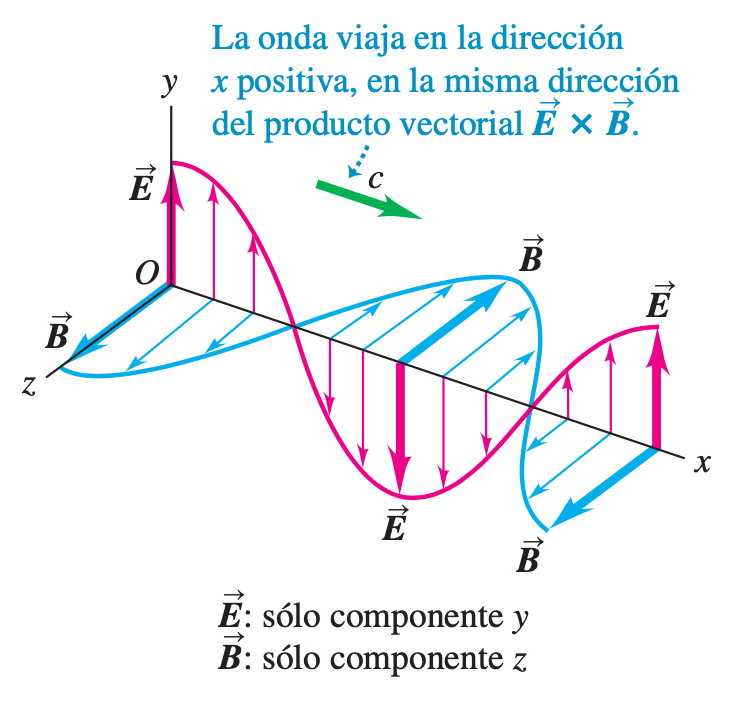
\includegraphics[scale=0.5]{fig/sinusoidal}
\caption{Representación de los campos eléctricos y magnéticos como funciones de x correspondientes a una onda electromagnética sinusoidal plana linealmente polarizada. Se ilustra una longitud de onda de la onda en el tiempo $t = 0$. Los campos se indican sólo para puntos a lo largo del eje $x$.}
\label{fig:sinusoidal}
\end{figure}

La figura \ref{fig:sinusoidal} muestra una onda electromagnética polarizada sinusoidal que viaja en la dirección $+x$. Observe que los campos eléctrico y magnético oscilan en fase: $\vec{E}$ es máximo donde $\vec{B}$ también lo es, y $\vec{E}$ es igual a cero donde $\vec{B}$ también vale cero. Advierta también que donde $\vec{E}$ está en la dirección $+y$, $\vec{B}$ tiene la dirección $+z$; y donde $\vec{E}$ está en la dirección $-y$, $\vec{B}$ está en la dirección $-z$. En todos los puntos, el producto vectorial $\vec{E}\times\vec{B}$ está en la dirección en que se propaga la onda .\footnote{En realidad, en una onda plana sinusoidal hay campos eléctricos y magnéticos en todos los puntos del espacio}.

Podemos describir las ondas electromagnéticas por medio de \textit{funciones de onda}, similar a como se hace para el caso de las ondas de una cuerda (ver sección \ref{cap:funcion-de-onda}). La ecuación (\ref{15.7}) es una forma de la función de onda para una onda transversal que viaja en la dirección $+x$ a lo largo de una cuerda estirada:

\begin{equation*}
y(x,t)=A\cos (kx-\omega t)
\end{equation*}

Dejemos que $E_y(x, t)$ y $B_z(x, t)$ representen los valores instantáneos de la componente $y$ de $\vec{E}$ y la componente $z$ de $\vec{B}$ en la figura \ref{fig:sinusoidal}, y sea que $E_{max}$ y $B_{max}$ representen los valores máximos, o amplitudes, de estos campos. De esta forma, las funciones de onda para la onda son

\begin{equation}\label{32.16}\marginnote{Onda electromagnética sinusoidal plana que se propaga en la dirección $+x$}
E_y(x,t)=E_{max}\cos (kx-\omega t)\qquad B_z(x,t)=B_{max}\cos (kx-\omega t)
\end{equation}

También es posible escribir las funciones de onda en forma vectorial:

\begin{equation}\label{32.17}
\boxed{\vec{E}(x,t)=\hat{j}E_{max}\cos (kx-\omega t)\qquad \vec{B}(x,t)=\hat{k}B_{max}\cos (kx-\omega t)}
\end{equation}

De (\ref{32.4}) se desprende que las amplitudes deben estar relacionadas mediante la expresión

\begin{equation}\label{32.18}\marginnote{Onda ekectromagnética en el vacío}
\boxed{E_{max}=cB_{max}}
\end{equation}

\begin{figure}
\centering
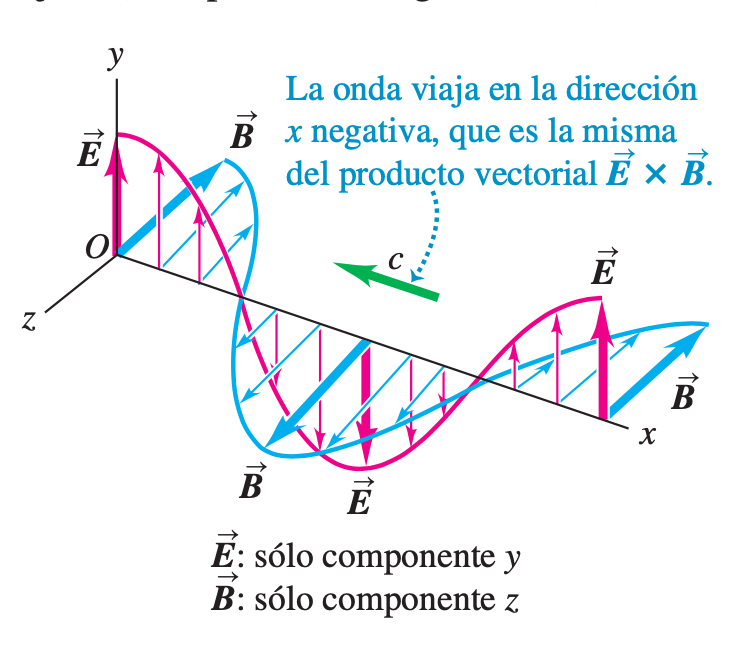
\includegraphics[scale=0.5]{fig/sinusoidal2}
\caption{Representación de una longitud de onda de una onda electromagnética sinusoidal plana linealmente polarizada, que viaja en la dirección $x$ negativa en el instante $t = 0$.}
\label{fig:sinusoidal2}
\end{figure}

La figura \ref{fig:sinusoidal2} muestra los campos eléctrico y magnético de una onda que viaja en la dirección $x$ negativa. Las funciones de onda correspondientes a esta onda son

\begin{equation}\label{32.19}\marginnote{Onda electromagnética sinusoidal plana, que se propaga en la dirección $-x$}
E_y(x,t)=E_{max}\cos (kx+\omega t)\qquad B_z(x,t)=-B_{max}\cos (kx+\omega t)
\end{equation}

\section{Energía y cantidad de movimiento de las ondas electromagnéticas}
Es un hecho muy conocido que hay energía asociada con las ondas electromagnéticas; piense en la energía de la radiación solar. 

Sabemos que en una región de espacio vacío donde están presentes los campos $\vec{E}$ y $\vec{B}$ la densidad total de energía $u$ está dada por

\begin{equation}\label{32.23}
u=\frac{1}{2}\epsilon_0E^2+\frac{1}{2\mu_0}B^2
\end{equation}

Para las ondas electromagnéticas en el vacío, las magnitudes $E$ y $B$ están relacionadas por

\begin{equation}\label{32.24}
B=\frac{E}{c}=\sqrt{\epsilon_0\mu_0}E
\end{equation}

Al combinar (\ref{32.23}) y (\ref{32.24}) también se puede expresar la densidad de energía $u$ en una onda electromagnética simple en el vacío como

\begin{equation}\label{32.25}
u=\frac{1}{2}\epsilon_0E^2+\frac{1}{2\mu_0}(\sqrt{\epsilon_0\mu_0}E)^2=\epsilon_0E^2
\end{equation}

Esto demuestra que en el vacío, la densidad de energía asociada con el campo $\vec{E}$ en nuestra onda simple es igual a la densidad de energía del campo $\vec{B}$. En general, la magnitud del campo eléctrico $E$ es función de la posición y el tiempo, igual que para la onda sinusoidal descrita por las ecuaciones (\ref{32.16}); así, la densidad de energía $u$ de una onda electromagnética, dada por la ecuación (\ref{32.25}), también depende en general de la posición y el tiempo.

\subsection{Flujo de energía electromagnética y el vector de Poynting}
Las ondas electromagnéticas como las que hemos descrito son ondas que \textit{viajan} y transportan energía de una región a otra. Esta transferencia de energía se puede describir en términos de la energía transferida \textit{por unidad de tiempo por unidad de área de sección transversal, o potencia por unidad de área}, para un área perpendicular a la dirección en que viaja la onda.

\begin{figure}
\begin{center}
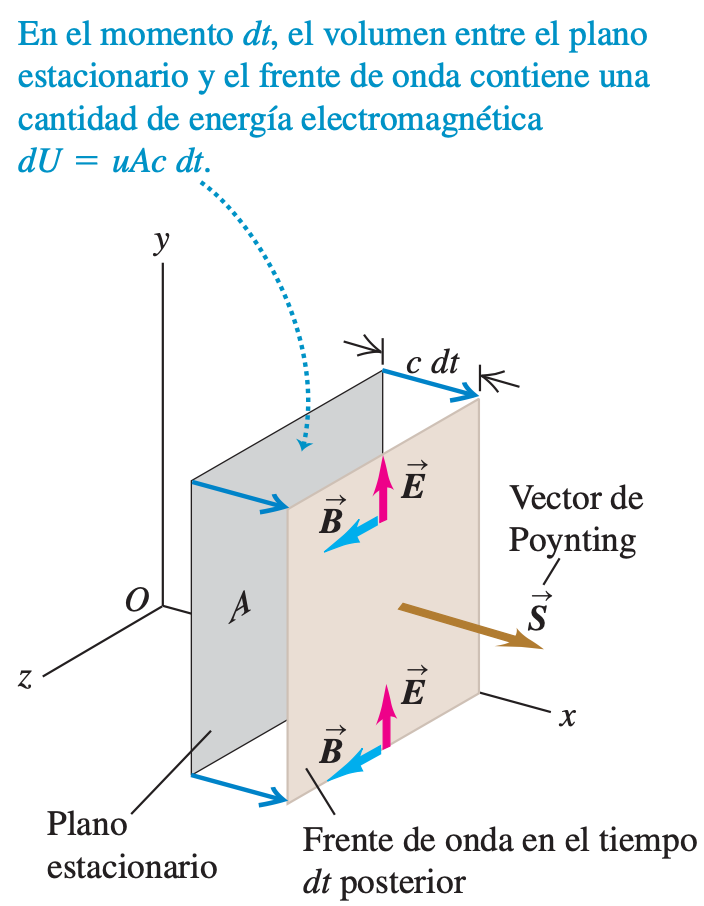
\includegraphics[scale=0.5]{fig/3217}
\caption{Frente de onda en el momento $dt$ después de haber pasado a través del plano estacionario con área $A$}
\label{fig:32.17}
\end{center}
\end{figure}


Para ver cómo se relaciona el flujo de energía con los campos, considere un plano estacionario, perpendicular al eje $x$, que coincida con el frente de onda en cierto momento. En un tiempo dt después de eso, el frente de onda se desplaza una distancia $dx = c\, dt$ hacia la derecha del plano. Si se considera un área $A$ sobre este plano estacionario (figura \ref{fig:32.17} ), advertimos que la energía del espacio a la derecha de esta área debió haber pasado a través del área para llegar a la nueva ubicación. El volumen $dV$ de la región en cuestión es el producto del área de la base $A$ por la longitud $c\, dt$, y la energía $dU$ de esta región es el producto de la densidad de energía $u$ por este volumen: $$dU=u\, dV=(\epsilon_0E^2)(Ac\, dt)$$

Esta energía pasa a través del área $A$ en el tiempo $dt$. El flujo de energía por unidad de
tiempo por unidad de área, que llamaremos $S$, es

\begin{equation}\label{32.26}
S=\frac{1}{A}\frac{dU}{dt}=\epsilon_0cE^2 \qquad \mbox{(en el vacío)}
\end{equation}

Las unidades de $S$ son energía por unidad de tiempo por uniad de área, o potencia por unidad de área.

Es posible definir una cantidad \textit{vectorial} que describa tanto la magnitud como la dirección de la tasa del flujo de energía:

\begin{equation}\label{32.28}\marginnote{Vector de Poynting en el vacío}
\boxed{\vec{S}=\frac{1}{\mu_0}\vec{E}\times\vec{B}}
\end{equation}

El vector $\vec{S}$ se denomina \textbf{vector de Poynting}. Su dirección es la misma en que se propaga la oinda. Como $\vec{E}$ y $\vec{B}$ son perpendiculares, la magnitud de $\vec{S}$ es $S=EB/\mu_0$; según (\ref{32.26}), éste es el flujo de energía por unida de área y por unidad de tiempo a través de un área de sección trnasversal perpendicular a la dirección de propagación. El flujo total de energía por uniad de tiempo (potencia $P$) hacia fiera de cualquier superficie cerrada es la integral de $\vec{S}$ sobre la superficie: $$P=\oint \vec{S}\cdot d\vec{A}$$. 

En el caso de las ondas sinosoidales, los campos eléctricos y masgnéticos en un ounto cualquiera varían en el tiempo, por lo que el vector de Poynting en cualquier punto también es función del tiempo. Puesto que las frecuencias de las ondas electromagnéticas comunes son muy altas, la variación en el tiempo del vector Poynting es tan rápida que lo más apropiado es examinar su valor \textit{medio}. La magnitud del valor medio de $\vec{S}$ en un punto recibe el nombre de \textbf{intensidad} de la radiación en ese punto. Veamos cuál es la intensiad de la onda sinosoidal descrita por (\ref{32.17}). Primero sustituimos $\vec{E}$ y $\vec{B}$ en (\ref{32.28}):

\begin{align*}
\vec{S}(x,t)&=\frac{1}{\mu_0}\vec{E}(x,t)\times\vec{B}(x,t) \\
&=\frac{1}{\mu_0}[\hat{j}E_{max}\cos(kx-\omega t)]\times [\hat{k}B_{max}\cos(kx-\omega t)]
\end{align*}

El producto vectorial de los vectores unitarios $\hat{j}\times \hat{k}=\hat{i}$, y $\cos^2(kx-\omega t)$ nunca es negativo, por lop que $\vec{S}(x,t)$ siemore apunta en la dirección $x$ positiva (la dirección de propagación de la onda). La componente $x$ del vector de Poynting es

\begin{equation*}
S_x(x,t)=\frac{E_{max}B_{max}}{\mu_0}\cos^2(kx-\omega t)=\frac{E_{max}B_{max}}{2\mu_0}[1+\cos 2(kx-\omega t)]
\end{equation*}

El valor medie del tiempo de $\cos 2(kx-\omega t)$ es igual a cero porque, en cualquier punto, es positivo durante la mitad de un ciclo y negtivo durante la otra mitad. Por lo tanto, el valor medio del vector de Poynting en un ciclo completo es $\vec{S}_{med}=\hat{i}S_{med}$, donde $$S_{med}=\frac{E_{max}B_{max}}{2\mu_0}$$

Es decir, la magnitud del valor medio de $\vec{S}$ para una onda siusoidal (la intensidad $I$ de la onda) es $\frac{1}{2}$ del valor máximo. Con base en las relaciones $E_{max}=B_{max}c$ y $\epsilon_0\mu_0=1/c^2$, podemos expresar la intensidad en varias formas equivalentes:

\begin{align*}\label{32.29}\marginnote{Intensidad de una onda sinusoidal en el vacío}
I&=S_{med}=\frac{E_{max}B_{max}}{2\mu_0}=\frac{E^2_{max}}{2\mu_0} \\
&=\frac{1}{2}\sqrt{\frac{\epsilon_0}{\mu_0}}E^2_{max}=\frac{1}{2}\epsilon_0cE^2_{max}
\end{align*}

Se invita al lectro a que compruebe que es estas expresiones son equivalentes.

En el caso de una onda que viaja en la dirección $-x$, el vector de Poynting tiene la dirección $-x$ en todos los puntos, pero su magnitud es la misma que en el caso de una onda que viaja en la dirección $+x$.

A lo largo de este análisis hemos considerado sólo ondas electromagnéticas que se propagan en el vacío. Sin embargo, si las ondas viajan en un medio dieléctrico, debem modificarse las expresiones para densidad de energía [(\ref{32.23})], el vector de Poynting [(\ref{32.28})] y la intensidad de una onda sinusoidal [(\ref{32.29})]. Los cambios requeridos son muy sencillos: basta con sustituir $\epsilon_0$ por la permitividad $\epsilon$ del dieléctrico, $\mu_0$ por la permitividad $\mu$ del dieléctrico, y $c$ por la rapidez $v$ de las ondas electromagnéticas en el dieléctrico. De manera sorpendente, las densidades de energía en los campo $\vec{E}$ y $\vec{B}$ son iguales incluso en un dieléctrico.




















